\scanpage{90}
% manuscript lines 1–2
\diagram{\begin{tikzcd}[ampersand replacement=\&,row sep=tiny]
 B\arrow[d,dash,very thick]\&M\&\deleted{\text{Coh. Mac}}\\ A\&\&
\end{tikzcd}}

% manuscript lines 2
\[
\operatorname{prof}M_y\deleted{\leq}=\mathop{\mathrm{Inf}}_{z\leftrightarrow y}\operatorname{prof}M_z
\geq\mathop{\mathrm{Inf}}_z\deleted{\dim M_z,k}\operatorname{Inf}(\dim M_z,k)
\]

% manuscript lines 3
\deleted{$\unsure{M}$} \deleted{$M_y\leq$ \unsure{on ait} $\operatorname{Inf}$}

% manuscript lines 3–4
\diagram{\begin{tikzcd}[ampersand replacement=\&,row sep=tiny]
B\arrow[d,dash]\&\text{\uline{normal}}\\ A\&{}
\end{tikzcd}}

% manuscript lines 4–5
$S_2$ comme \deleted{\unsure{anneau}}, \unsure{anneau}, mais pas comme module

% manuscript lines 6
\[
 B/fB\simeq\unsure{0|O|\mathcal O}\,\unsure{0|{}_{X_0}}
\]

% manuscript lines 6–9
\figure{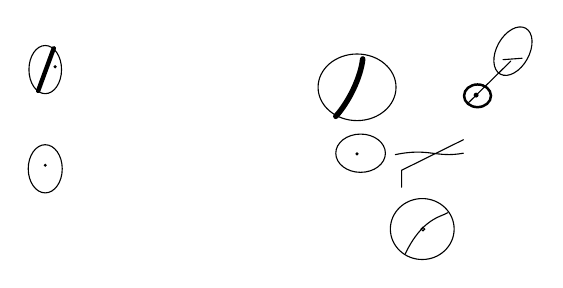
\begin{tikzpicture}[x=.9cm,y=.9cm,line cap=round]
\draw (0,2.9) ellipse (.23 and .34); \draw[line width=1.6pt](-.1,2.6)--(.12,3.2); \fill(.14,2.94)circle(.025);
\draw (0,1.5) ellipse (.24 and .34); \fill (0,1.55)circle(.023);
\draw (4.4,2.65) ellipse (.55 and .47); \draw[line width=2pt](4.1,2.24)..controls(4.28,2.44)and(4.45,2.78)..(4.48,3.05);
\draw (4.45,1.72) ellipse (.35 and .27); \fill (4.4,1.71)circle(.025);
\draw (5.32,.65) ellipse (.45 and .43); \draw (5.08,.3)..controls(5.32,.8)and(5.58,.82)..(5.68,.88); \draw(5.33,.65)circle(.025);
\draw (5.03,1.24)--(5.03,1.48)--(5.9,1.91); \draw(4.94,1.7)..controls(5.42,1.8)and(5.51,1.65)..(5.9,1.72);
\draw[line width=.9pt](6.1,2.53) ellipse (.19 and .16); \fill(6.08,2.54)circle(.035); \draw(5.97,2.43)--(6.57,3.02); \draw[rotate around={-29:(6.6,3.16)}](6.6,3.16) ellipse (.23 and .37); \draw(6.46,3.04)--(6.73,3.06);
\end{tikzpicture}}

% manuscript lines 7–9
\diagram{\begin{tikzcd}[ampersand replacement=\&,row sep=tiny]
B\arrow[d,dash,very thick]\&B\subset A^{\unsure{r|n}}\\
A\& A^n\qquad B/fB\subset(A/fA)^r
\end{tikzcd}}

% manuscript lines 9
\figure{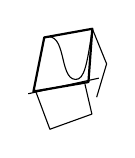
\begin{tikzpicture}[scale=.55,line join=round]
\draw[thick] (0,0)--(.25,1.25)--(1.36,1.45)--(1.27,.22)--cycle;
\draw (.04,.04)--(.38,-.87)--(1.35,-.52)--(1.19,.17); \draw (1.36,1.45)--(1.69,.64)--(1.46,-.13);
\draw (.25,1.25) .. controls (.78,1.42) and (.58,.3) .. (.97,.28) .. controls (1.18,.27) and (1.24,.64) .. (1.36,1.45);
\draw(-.12,-.05)--(1.51,.31);
\end{tikzpicture}}

% manuscript lines 10–11
\diagram{\begin{tikzcd}[ampersand replacement=\&,row sep=tiny]
B\arrow[d,dash,very thick]\&B/fB\arrow[r]\&(A/fA)^r\\ A\&\&
\end{tikzcd}}

% manuscript lines 11
\deleted{\illegible{2}}

% manuscript lines 12–13
\diagram{\begin{tikzcd}[ampersand replacement=\&,row sep=tiny]
B\&M\&M\ S_k\arrow[r,Rightarrow,"{?}"]\&M_{[\,]}\text{ est }(S_k)\\ A\&{}\&\deleted{\unsure{f_1}}\&{}
\end{tikzcd}}

% manuscript lines 14–16
$\mathfrak p\in\unsure{A|\mathfrak A}$\qquad $\dim A_{\mathfrak p}\leq k\Longrightarrow\dim B_{\mathfrak p}\leq k$ donc $M_{\mathfrak p}$ est Coh. Mac sur $B_{\mathfrak p}$, donc $M_{\mathfrak p}$ est Coh. Mac \uline{mais pas comme mod sur $A$}

% manuscript lines 15–17
\diagram{\begin{tikzcd}[ampersand replacement=\&,row sep=tiny]
B_{\mathfrak q}\&M_{\mathfrak q}\&\dim M_{\mathfrak q}\quad\operatorname{prof}M_{\mathfrak q}\\ A_{\mathfrak p}\&{}\&{}
\end{tikzcd}}

% manuscript lines 16–18
\uline{$B$ est Coh. Mac} comme anneau, $\dim B_{\mathfrak q}=\operatorname{prof}^{\prime\prime}$

% manuscript lines 19–20
\[
\begin{aligned}
\operatorname{prof}M_{\mathfrak p}\geq\operatorname{Inf}(k,\deleted{\unsure{A}}\dim M_{\mathfrak p})&\Longleftrightarrow\operatorname{prof}\widehat M_{\mathfrak p}\geq\operatorname{Inf}(k,\dim\widehat M_{\mathfrak p})\\
&\operatorname{prof}\widehat M_{\mathfrak q_i}^{\prime\prime}\geq\operatorname{Inf}(k,{}^{\prime\prime}\dim\widehat M_{\unsure{\mathfrak p|\mathfrak q_i}})
\end{aligned}
\]

% manuscript lines p1–p3
% margin note written sideways
\margin{$\mathfrak a=fA+gA\supseteq\mathfrak p^n\quad(\exists n)$\quad $\mathfrak a(\mathfrak m)$\quad $\mathfrak p$ \quad complete intersection of dim $\geq4$ $\Longrightarrow\operatorname{Pic}(X-\mathfrak a)=0$}

% manuscript lines p4–p6
% margin note written sideways
\margin{$A_f$ \unsure{normal|non local} $A$ UFD $\Longleftrightarrow$ 1) $A_{\mathfrak p}$ is UFD\quad $\mathfrak p\ne\mathfrak a$ 2) $\operatorname{Pic}(X-\mathfrak a)=0$ \quad $A$ complete intersection of dim $\geq3$}

% manuscript lines p7–p8
% margin note written sideways
\margin{$f\in\unsure{\mathfrak p|A}\quad A'$ non zero divisor \quad Thm: principal \unsure{theorem} holds. \unsure{If|I.e.} \unsure{Assume} \unsure{possibly} \unsure{only} $\unsure{\pi_1|\operatorname{Pic}}(\unsure{X|A})=0$. \quad $\unsure{B|R}=A/f$}

% manuscript lines p9–p13
% margin note written sideways
\margin{$Y'\quad \boxed X$ \quad $Y'=Y-\mathfrak a$, $X'=X-\mathfrak a$ \quad 1) if $\forall x\in X'-Y'$, $\dim\bar x=1\Longrightarrow\operatorname{depth} A_x\geq3$, $\varphi$ is \uline{injective}. 2) if $\forall x\in X'-Y'$, $\dim\bar x=1\Longrightarrow\operatorname{depth} A_x\geq\unsure{4}$ and if $\operatorname{Pic}(\operatorname{Spec} A_x-\{x\})=0$ $\Longrightarrow\varphi$ is bij}

% manuscript lines p10–p12
% margin note written sideways
\diagram{\begin{tikzcd}[ampersand replacement=\&,column sep=large]
\pi_1(Y')\arrow[r,"\varphi"]\&\pi_1(X')\\
\operatorname{Pic}(X')\arrow[r,"\varphi"]\&\operatorname{Pic}(Y')
\end{tikzcd}}
% archive sheet number: 89

